\documentclass[12pt,a4paper]{report}

\usepackage[backend=biber, style=ieee]{biblatex}
\addbibresource{literature.bib}

\usepackage[utf8]{inputenc}
\usepackage[T1]{fontenc}
\usepackage[ngerman]{babel}
\usepackage{lmodern}
\usepackage{enumitem}
\usepackage{graphicx}
\usepackage{tabularx}
\usepackage{float}
\usepackage[onehalfspacing]{setspace}
\usepackage{microtype}
\usepackage{parskip}
\usepackage{minted}

\usepackage{xcolor}
\newcommand{\todo}[1]{\colorbox{red}{\textbf{TODO: #1}}\\}
\newcommand{\question}[1]{\colorbox{yellow}{\textbf{QUESTION: #1}}\\}
\newcommand{\xeno}[1]{\colorbox{pink}{\textbf{TODO XENO: #1}}\\}
\newcommand{\gideon}[1]{\colorbox{green}{\textbf{TODO GIDEON: #1}}\\}

\begin{document}

\tableofcontents
\newpage


\section{Health Companion}

Gesundheitsdaten können wertvolle Zusatzinformationen zur Entwicklerzufriedenheit liefern. Sie ergänzen subjektive Stimmungsangaben
um objektive Messwerte, die Rückschlüsse auf Belastung und Erholung ermöglichen. Durch die Anbindung an etablierte Schnittstellen
wie Apple Health Kit oder Garmin Health API lassen sich Metriken wie Schlafqualität, Herzfrequenz oder Stressindikatoren
automatisiert erfassen. Diese Daten bilden zusammen mit den Prozess- und Zufriedenheitsmetriken eine erweiterte Grundlage, um
Korrelationen zwischen physischem Wohlbefinden und Arbeitszufriedenheit zu erkennen und gezielte Massnahmen abzuleiten.

\subsection{Quellen und Schnittstellen für Gesundheitsdaten}

Für die Integration von Gesundheitsdaten wurden mehrere Optionen geprüft. Im Mittelpunkt standen die Garmin Health API sowie Apple
Health Kit. Beide Quellen decken relevante Metriken wie Schritte, Herzfrequenz, Schlaf und Stress/HRV ab, unterscheiden sich jedoch
deutlich hinsichtlich Zugangsmodell, Datenschutzmechanismen, Integrationsaufwand und Eignung für nicht-kommerzielle
Forschungsprojekte.

\begin{description}
  \item[Garmin Health API] Die Garmin Health API stellt über eine REST-Schnittstelle umfangreiche Tages- und Aktivitätsmetriken
    bereit. Die Daten werden in der Regel nach dem Gerätesync via über die Mobile Applikation von Garmin bereitgestellt und in
    JSON ausgeliefert. die Plattform unterstützt Pull- und Push-Modelle, sodass auch eine ereignisgetriebene Integration möglich
    ist. Der Zugang ist für genehmigte Business-Developer vorgesehen. Für die kommerzielle Nutzung fallen in der Regel
    Lizenzgebühren an. Diese geschäftliche Ausrichtung sowie die erforderliche formale Zulassung machen die direkte Nutzung für
    ein kleines, nicht-kommerzielles Forschungsprojekt unpassend. Zwar existieren Forschungsprogramme und Partnerlösungen rund um
    Garmin, diese sind jedoch üblicherweise an formelle Kooperationen, Vertragsaufwände und teils Kosten gebunden, was die
    Umsetzungshürde erhöht \cite{garmin_healthapi_2025}.
  \item[Apple Health Kit] Health Kit dient auf iOS als zentrales, lokales Datenrepository für Gesundheits- und Fitnessdaten von
    iPhone, Apple Watch und angebundenen Geräten/Apps. Der Zugriff erfolgt feingranular pro Datentyp und erfordert stets explizite
    Nutzerzustimmung (Lesen/Schreiben getrennt). Daten liegen verschlüsselt auf dem Gerät. Apps erhalten nur Zugriff auf die
    explizit freigegebenen Kategorien. Für die Integration stehen dokumentierte APIs und Query-Muster zur Verfügung. Eine
    serverseitige Drittplattform ist nicht erforderlich, wodurch Architektur, Betrieb und Datenschutzfolgenabschätzung vereinfacht
    werden \cite{apple_healthkit_2025}.
\end{description}

Da die Garmin Health API primär für kommerzielle Anwendungen vorgesehen ist und der beantragte Zugang für dieses Projekt nicht
gewährt wurde, wurde Apple Health Kit als geeignetere Datenquelle ausgewählt. Für die Umsetzung bedeutet dies, dass eine
iOS-Anwendung entwickelt wird, die die relevanten Daten aus Apple HealthKit ausliest und an Yappi überträgt.

\subsection{Daten aus HealthKit auslesen}

Um relevante Gesundheitsmetriken automatisiert zu erfassen, nutzt die iOS-Anwendung die von Apple bereitgestellte
HealthKit-Schnittstelle. In diesem Kapitel wird der Zugriff auf die Schrittzählungsdaten erklärt, die anderen Metriken werden
auf die gleiche Art und Weise implementiert. 

Der Zugriff auf HealthKit-Daten erfordert die explizite Zustimmung des Nutzers für jede einzelne Datenkategorie. Beim ersten Start
der App wird daher eine Berechtigungsanfrage angezeigt, in der der Zugriff auf Schrittzählungsdaten 
(\texttt{HKQuantityTypeIdentifier.stepCount}) angefordert wird. Erst nach Bestätigung durch den Nutzer beginnt die App mit der
Erfassung.

Die Umsetzung der Datenerfassung erfolgt über eine Kombination aus einem \texttt{HKObserverQuery} und zeitlich begrenzten 
\texttt{HKStatisticsQuery}-Abfragen. Der \texttt{HKObserverQuery} registriert sich auf Änderungen in den beobachteten Metriken und
wird von HealthKit automatisch ausgelöst, sobald neue Daten vorliegen. Für jede Verarbeitung wird der zuletzt verarbeitete 
Zeitraum gespeichert, sodass bei der nächsten Abfrage nahtlos an dieser Stelle fortgesetzt werden kann, ohne bereits erfasste
Daten erneut zu verarbeiten.

Die gesammelten Daten werden anschliessend über einen API-Endpoint an das Backend der Yappi-Plattform übertragen und dort
gespeichert. Dadurch stehen sie zentral zur Verfügung und können gemeinsam mit anderen erfassten Metriken ausgewertet werden. 

\subsection{Daten an Yappi übertragen}

Um die Verarbeitung auf Serverseite zu vereinfachen und die Erweiterbarkeit auf weitere Metriken zu ermöglichen, werden die Daten
in einer einheitlichen JSON-Struktur übertragen. Diese enthält zum einen den Typ der Metrik (\texttt{metric}), zum anderen ein Array
von Messwerten, das für jeden Eintrag den erfassten Zeitraum sowie den zugehörigen Wert enthält. Die Zeiträume werden im
Format \texttt{yyyy-MM-dd~HH:mm/yyyy-MM-dd~HH:mm} angegeben, um sowohl das Start- als auch das Enddatum einer Messung eindeutig
zu definieren.

\begin{verbatim}
{
    "metric": "STEPS",
    "data": [
        {
            "timeRange": "yyyy-MM-dd HH:mm/yyyy-MM-dd HH:mm",
            "value": steps
        },
        {
            "timeRange": "2025-08-06 08:00/2025-08-06 09:00",
            "value": 38
        }
    ]
}
\end{verbatim}

Diese Struktur erlaubt eine konsistente Verarbeitung unabhängig von der Art der Metrik und bildet die Grundlage für die
serverseitige Validierung, Speicherung und spätere Analyse. Sie kann ohne Anpassungen um weitere Metriken erweitert werden,
indem lediglich der Wert von \texttt{metric} angepasst und das \texttt{data}-Array mit den entsprechenden Messpunkten befüllt
wird.

Im folgenden Abschnitt werden die notwendigen Anpassungen im Backend und in der Datenbank erläutert, um die empfangenen
Messdaten zu verarbeiten und dauerhaft zu speichern.

\subsubsection{Backend}

Für die Verarbeitung der eingehenden Gesundheitsdaten wurde im Backend ein Controller mit zugehörigem Service und Repository
implementiert. 

Der Controller stellt einen REST-Endpunkt bereit, über den die Companion-App die Daten im beschriebenen JSON-Format an die
Plattform übermitteln kann. 

\begin{description}
  \item \texttt{POST /companion/health} \\
        Nimmt Gesundheitsdaten im definierten JSON-Format entgegen und speichert sie für den authentisierten Nutzer. 
        Bereits vorhandene Einträge im angegebenen Zeitraum werden aktualisiert, andernfalls werden neue Einträge angelegt. \\
        \textbf{Antworten:} \texttt{200 OK}, \texttt{400 Bad Request}, \texttt{401 Unauthorized}.
\end{description}

Die eingehenden Anfragen werden an den Service weitergeleitet, der die eigentliche Geschäftslogik übernimmt. Der Service prüft
zunächst, ob für den übermittelten Benutzer und die angegebene Metrik im gesendeten Zeitraum bereits ein Eintrag in der Datenbank
vorhanden ist. Falls ja, wird der bestehende Datensatz überschrieben, um stets den aktuellsten Stand zu gewährleisten. Falls kein
Eintrag vorhanden ist, wird ein neuer Datensatz angelegt.  

Das Repository kapselt den Zugriff auf die Datenbank und übernimmt das Einfügen sowie das Aktualisieren der Messwerte. Durch diese
Aufteilung in Controller, Service und Repository wird eine klare Trennung von Zuständigkeiten erreicht, was die Wartbarkeit und
Erweiterbarkeit der Implementierung erleichtert.

\subsubsection{Datenbankerweiterung}

Zur Speicherung der von der Companion-App übermittelten Gesundheitsdaten wurde das Datenbankschema um die Tabelle 
\texttt{health\_metric} erweitert. Diese Tabelle dient als generische Ablage für unterschiedliche Metriken. Durch diese Struktur
lassen sich weitere Gesundheitsmetriken ohne Schemaänderungen hinzufügen.  

\begin{table}[H]
\centering
\begin{tabular}{|l|l|p{9cm}|}
\hline
\textbf{Spalte} & \textbf{Datentyp} & \textbf{Beschreibung} \\
\hline
\texttt{id} & SERIAL & Primärschlüssel, auto-inkrementierend \\
\texttt{user\_id} & INTEGER & Fremdschlüssel auf \texttt{users.id} \\
\texttt{metric} & TEXT & Typ der Metrik (z.\,B. \texttt{STEPS}, \texttt{SLEEP}) \\
\texttt{start\_time} & TIMESTAMPTZ & Beginn des Messzeitraums \\
\texttt{end\_time} & TIMESTAMPTZ & Ende des Messzeitraums \\
\texttt{value} & NUMERIC & Messwert der Metrik \\
\texttt{created\_at} & TIMESTAMPTZ & Zeitpunkt der Erfassung in der Datenbank \\
\hline
\end{tabular}
\caption{Schema der Tabelle \texttt{health\_metric}}
\label{tab:health_metric_schema}
\end{table}

\subsection{Benutzeroberfläche der iOS App}

Nachfolgend wird die Benutzeroberfläche der iOS App vorgestellt. Die Benutzeroberfläche der iOS-Anwendung ist bewusst
minimalistisch gehaltet und darauf ausgelegt, den API-Key einmalig zu hinterlegen, ohne dass danach weitere Eingaben erforderlich
sind.

\begin{figure}[H]
  \centering
  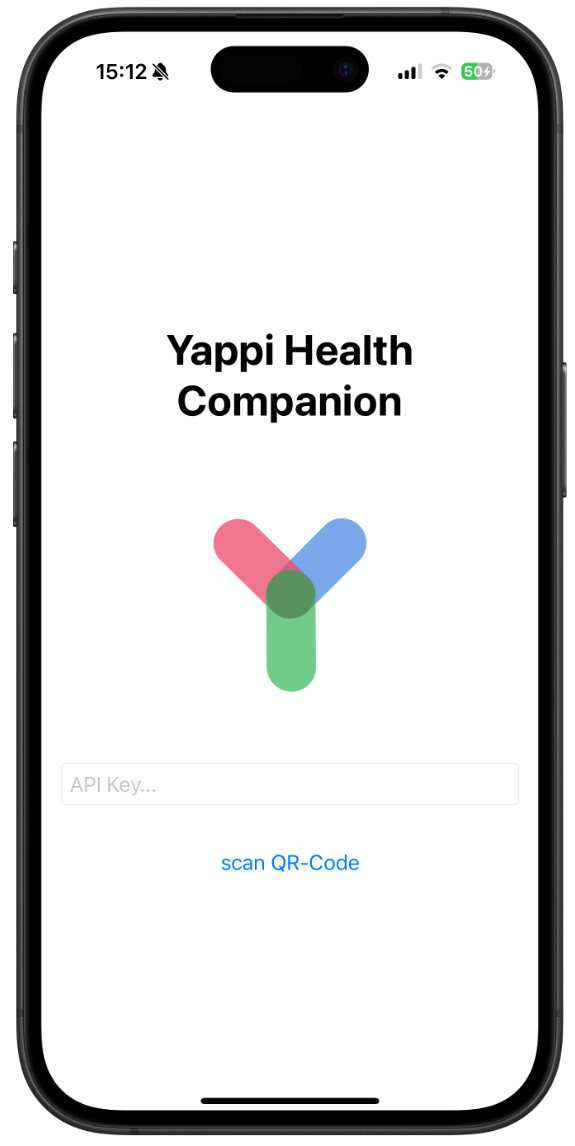
\includegraphics[height=0.5\textheight,keepaspectratio]{../figures/health-app.png}
  \caption{Benutzeroberfläche der iOS Health Companion App}
  \label{fig:health-app}
\end{figure}

Die Abbildung~\ref{fig:health-app} zeigt die Benutzeroberfläche der App. Für die Eingabe des API-Keys stehen mehrere Wege zur
Verfügung, entweder durch manuelle Eingabe oder durch das Scannen eines QR-Codes. Der integrierte QR-Code-Scanner öffnet sich im
Vollbildmodus, erkennt den Schlüssel automatisch und trägt ihn direkt in das Eingabefeld ein. Nach der Eingabe wird der API-Key
in den UserDefaults des Geräts gespeichert, sodass er bei späteren App-Starts automatisch geladen wird.

Die Verarbeitung der Gesundheitsdaten erfolgt vollständig im Hintergrund. Sobald neue Werte vorliegen, werden diese automatisch an
Yappi übertragen. Dadurch entfällt für den Nutzer jede manuelle Auslösung und der Betrieb der App erfordert keine zusätzliche
Interaktion.

\printbibliography

\end{document}
